\documentclass{article}
\usepackage{graphicx}
\usepackage{amsmath}
\title{\textbf{homework-01}}
\author{SixGod}
\date{\today}

\begin{document}
\maketitle

\section{Broken Chessboard and Jumping With Coins}
\subsection{Tiling a Damaged Checkerboard}

\begin{flushleft}
\textbf{Exercise 1.1.} \\
Firstly, we color the chessboard in black and white.\\
\begin{center}
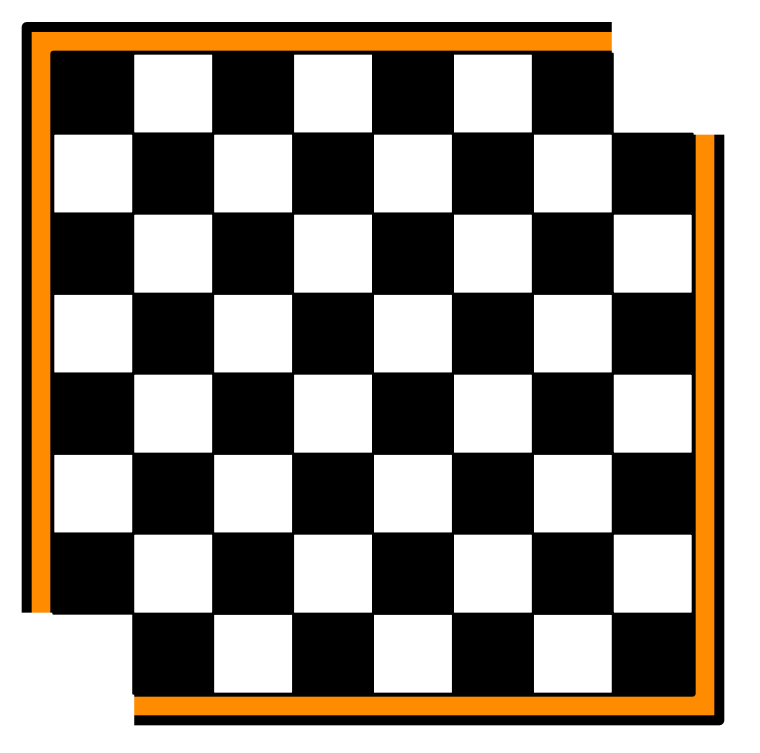
\includegraphics[scale=0.3]{1_1_1.png}
\end{center}
So now, we have 32 black squares and 30 white squares.\\
And if we put a tile in this chessboard, it will cover exactly a black square and a white squre, no matter how we put it.\\
So if we continue put tiles on it, we will have two black squares left in the end.\\
\begin{center}
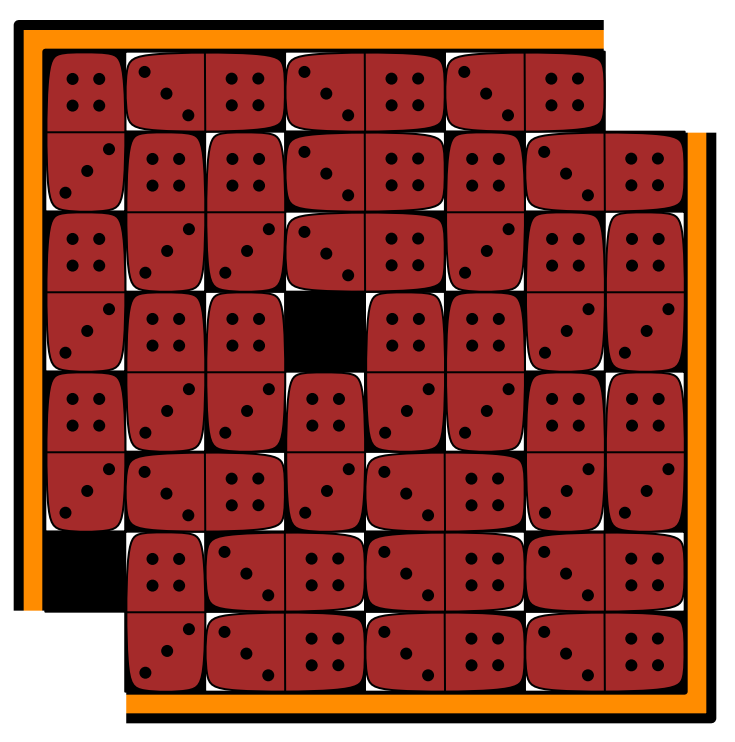
\includegraphics[scale=0.3]{1_1_2.png}
\end{center}
It means that whatever we do we will always get stuck because there are always two more black squares than white squares.\\
So it is obvious that we cannot tile this damaged chessboard.\\

\textbf{Exercise 1.2.} \\
...

\end{flushleft}
\subsection{Jumping with Coins}

\begin{flushleft}
\textbf{Exercise 1.3.} \\
Obviously, we have only two coins, so that each of them can only jump over the other one.
In this case, the distance between the two coins will never change. So we cannot increase the 
distance between the two coins.

\textbf{Exercise 1.4.} \\
When one coin jump over another one, like the picture below:
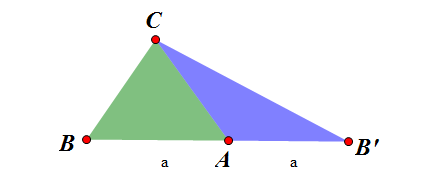
\includegraphics[scale=0.7]{1_3_1.png}\\
Obviously, we can find that $AB = AB'$,and this two triangles have a same height, so we get  $S_{\Delta ABC}$ = $S_{\Delta AB'C}$.\\
Considering that, however we jump the coin,the area of the triangle will never change.\\
So,we cannot start with an equilateral triangle and end up with a bigger equilateral triangle.

\textbf{Exercise 1.5.} \\
A coin is at a position $(x,y)\in\mathbf{R}^2$ .\\
we assume that in the begning the pos are (0,0),(0,1),(1,0),(1,1).\\
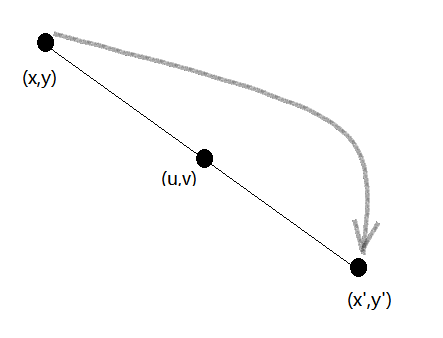
\includegraphics[scale=1]{1_5_1.png}\\
$(u,v)+(u,v)-(x,y)=(2u-x,2v-y)$\\
if $(u,v),(x,y)\in\mathbf{Z}^2$ , then $(2u-x,2v-y)\in\mathbf{Z}^2$.\\
Thus the coins will always be on an integer position.
Now let (x,y) be the position of a coin,\\
if $(x,y)\in\mathbf{Z}^2$, we can say coin is
$
\left\{\begin{array}{ll}
white & \textrm{while x+y is odd}\\
black & \textrm{while x+y is even}
\end{array} \right.
$
.\\
So, now the color of (x,y) is $x+y\mod2$, the color of (2u-x,2u-y) is $(2u-x)+(2v-y)\mod2=(x+y)\mod2$
,they are on the same color square.\\
Considering that, we put four coins on a chessboard like this:
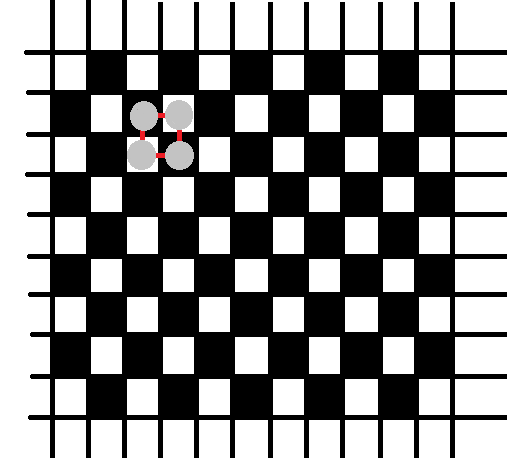
\includegraphics[scale=0.8]{1_5_2.png}\\
We can see there are two coins on white square and two on black square.\\
And if the side length of coin square becomes 2, it will look like this:
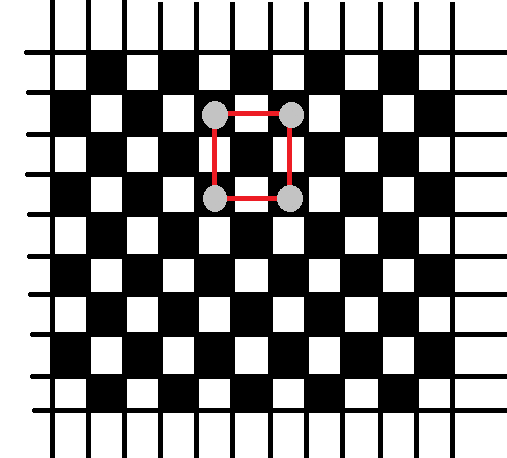
\includegraphics[scale=0.8]{1_5_3.png}\\
In this situation, all coins are on white (or black) square. 
But we have already proved that every coin's color will not change, so this pattern can never be achieved.

\textbf{Exercise 1.6.} \\
From the problem 1.5, we already know that the color of the coin will never change. So, if we want the two coins move to the same position, they must have same color, we might as well assume that color is black.\\
Like problem 1.5,assume that in the begning the pos are (0,0),(0,1),(1,0),(1,1).\\
        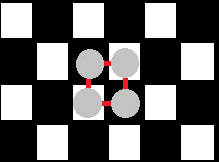
\includegraphics[scale=1]{1_6_1.png}\\
The black ones are (0,0),(1,1). Consider their x-coordinates, however we jump the coin, their x-coordinate will be 2k and 2m+1 (m,k are integers),the sum is 2(k+m)+1,which is an odd number\\
If we can move them to a same position, the sum of x-coordinate will be 2n (n is a integer),which is an even number.Obviously, it is contradictory to the conclusion we get above. If the color is white, it will be the same way to prove it.\\
So, we cannot achieve a position in which two coins are at the same position.\\


\textbf{Exercise 1.7.} \\
...

\textbf{Exercise 1.8.} \\
...

\end{flushleft}
\section{Exclusion-Inclusion}
\subsection{Sets}

\begin{flushleft}
\textbf{Exercise 2.1.} \\
...

\textbf{Exercise 2.2.} \\
...

\textbf{Exercise 2.3.} \\
...

\end{flushleft}
\section{Feasible Intersection Patterns}

\begin{flushleft}
\textbf{Exercise 3.1.} \\
...

\textbf{Exercise 3.2.} \\
...

\textbf{Exercise 3.3.} \\
...
\end{flushleft}
\end{document}